\documentclass[a4paper,12pt]{article}

% Поля страниц
\usepackage[left=2.5cm,right=2.5cm,
top=2cm,bottom=2cm,bindingoffset=0cm]{geometry}

% Рисунки
\usepackage{caption,floatrow}
\usepackage{floatrow,graphicx,calc}
\usepackage{wrapfig}

%Пакет дял таблиц   
\usepackage{multirow} 
\usepackage{array,tabularx,tabulary,booktabs} % Дополнительная работа с таблицами
\usepackage{longtable} 

%Отступ после заголовка    
\usepackage{indentfirst}

%%% Работа с русским языком
\usepackage{cmap}					% поиск в PDF
\usepackage{mathtext} 				% русские буквы в формулах
\usepackage[T2A]{fontenc}			% кодировка
\usepackage[utf8]{inputenc}			% кодировка исходного текста
\usepackage[english,russian]{babel}	% локализация и переносы

%%% Дополнительная работа с математикой
\usepackage{amsmath,amsfonts,amssymb,amsthm,mathtools} % AMS

%% Номера формул
\mathtoolsset{showonlyrefs=true} % Показывать номера только у тех формул, на которые есть \eqref{} в тексте.

\usepackage{icomma} % "Умная" запятая: $0,2$ --- число, $0, 2$ --- перечисление

%% Шрифты
\usepackage{euscript}	 % Шрифт Евклид
\usepackage{mathrsfs} % Красивый матшрифт

%% Перенос знаков в формулах (по Львовскому)
\newcommand*{\hm}[1]{#1\nobreak\discretionary{}
{\hbox{$\mathsurround=0pt #1$}}{}}

%%% Заголовок
\author{Александр Плукчи}
\title{Лабораторный практикум}
\date{\today}

\begin{document} % конец преамбулы, начало документа
	\textbf{Работа № 3.2.5}
	
	\textbf{\Large{Вынужденные колебания в электрическом контуре}}
	
	\textbf{В работе используются:} генератор звуковой частоты (ЗГ), осциллограф (ЭО), вольтметр, частотомер, ёмкость, индуктивность, магазин сопротивлений, универсальный мост.

	\section*{Ход работы}
		\subsection*{Исследование резонансных кривых}
			\begin{enumerate}
				\item Рассчитаем резонансную частоту контура $\nu_0 = 1/(2\pi\sqrt{LC})$.
				\item Снимем зависимость показаний вольтметра $U$ от показаний частотомера $\nu$ при $R = 0$ Ом и $R = 100$ Ом. 
				\item Построим график зависимости $U/U_0 = f(\nu/\nu_0)$.
			\end{enumerate}
		\subsection*{Процессы установления и затухания колебаний}
			\begin{enumerate}
				\item Для расчёта добротности по скорости нарастания (затухания) амплитуды измерим амплитуды колебаний всех периодов для $R = 0$ Ом и $R = 100$ Ом и построим графики в условных единицах (по фотографиям экрана осциллографа).
				\item По отношению соседних амплитуд вычислим добротность: $Q = \frac{\pi}{\ln{(U_k/U_{k+1})}}$.
				\item Измерим активное сопротивление $R_L$ и индуктивность $L$ магазина индуктивностей с помощью измерителя LCR на частотах 50 Гц, 500 Гц и 1500 Гц.
			\end{enumerate}
		
		
	\section*{Обработка результатов}
		Полученные графики и таблицы представлены ниже:
		\begin{table}[H]
			\caption{Данные.}
			\label{table:D}
			\begin{tabular}{|c|c|c|c|}
				\hline
				$\nu_0$, Гц & $L$, мГн & $C$, мкФ & $R_L$, Ом \\ \hline
				1567 & 100,01 & 0,1 & 25,58 \\ \hline
			\end{tabular}
		\end{table}
		\begin{figure}
			\ffigbox{\label{ris:unu}}{\includegraphics[width=13cm, height=8cm]{u(nu).pdf}}
		\end{figure}
		\begin{table}[H]
			\caption{Добротность.}
			\label{table:Q}
			\begin{tabular}{|c||c|c|c|c|}
				\hline
				\multirow{2}{*}{$R$, Ом}  & \multicolumn{4}{c|}{$Q$} \\ \cline{2-5}
				& $\omega_0/\Omega$ & нараст & убыв & $f(LCR)$ \\
				\hline \hline
				0  & $38,9 \pm 1,5$  & --- & $34,5 \pm 5,4$ & $39,1 \pm 0,8$ \\
				100  & $7,7 \pm 0,6$ & $7,9 \pm 0,9$ & $8,03 \pm 0,6$ & $7,96 \pm 0,16$ \\ \hline
			\end{tabular}
		\end{table}
		\begin{minipage}{.48\textwidth}
			\centering
			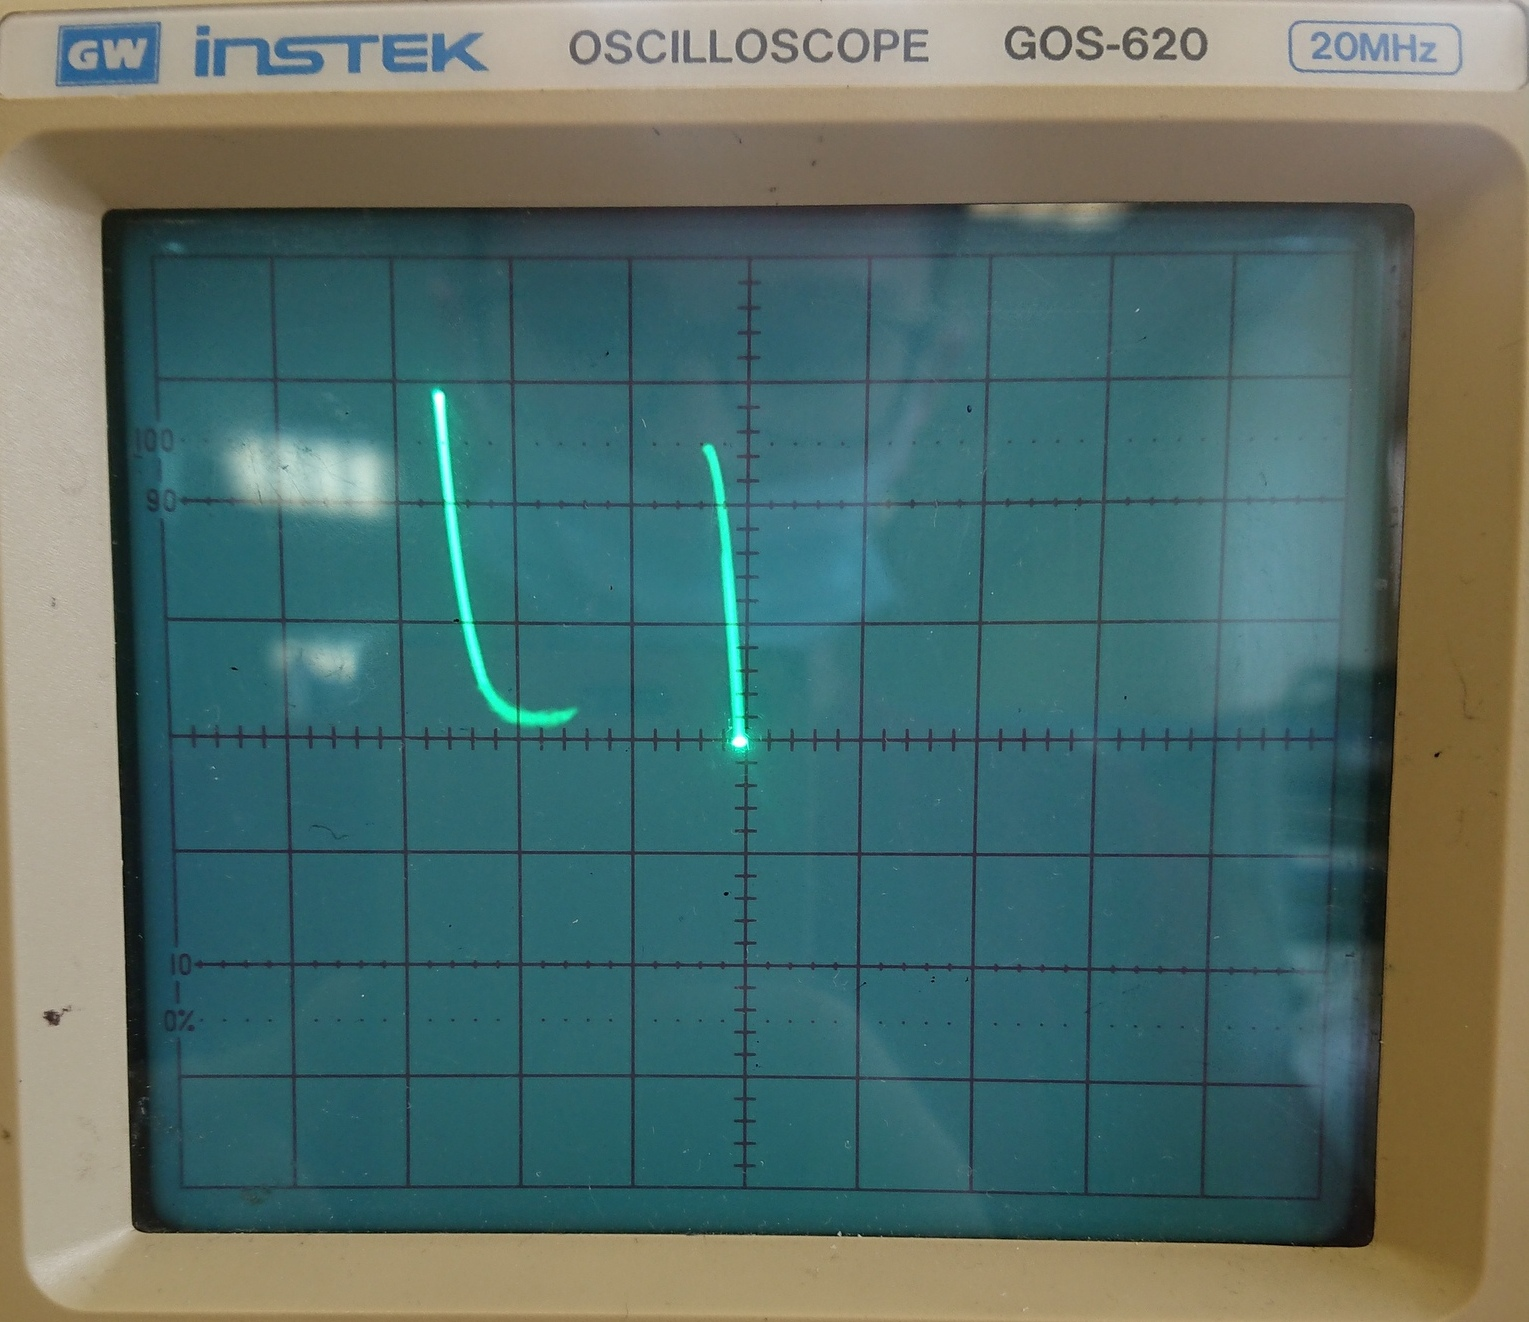
\includegraphics[width=7cm, height=5cm]{osc1.pdf}
		\end{minipage}
		\begin{minipage}{.48\textwidth}
			\centering
			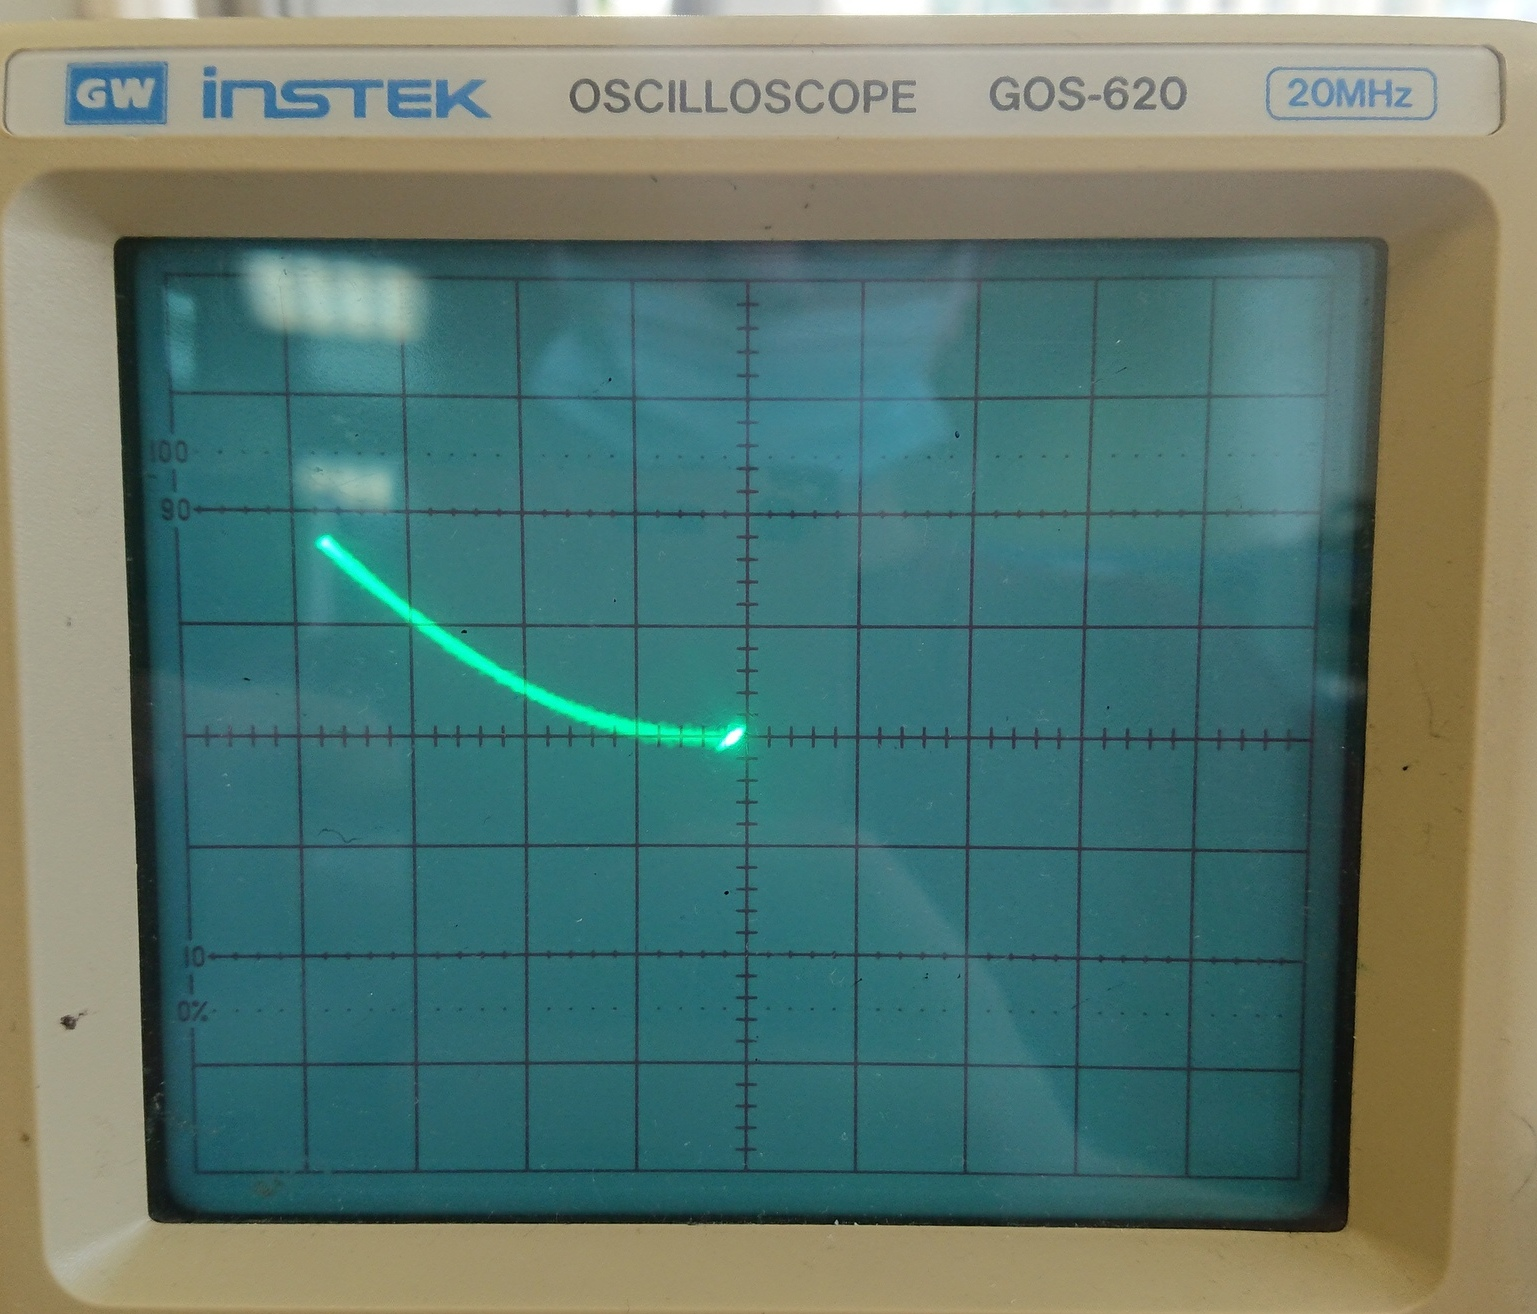
\includegraphics[width=7cm, height=5cm]{osc2.pdf}
		\end{minipage}
		\begin{figure}[H]
			\caption{Пики колебаний.}
			\includegraphics[width=7cm, height=5cm]{osc3.pdf}
		\end{figure}
		
		
		\section*{Вывод}
			Таким образом, мы вычислили добротность контура при различных сопротивлениях резистора различными способами: $Q = 39,1 \pm 0,8$ при $R = 0$ Ом и $Q = 7,96 \pm 0,16$ при $R = 100$ Ом. Результаты вычислений различными способами в пределах погрешности совпадают.
			
\end{document} % конец документа

